% ChargeShield-FL --- DSN 2027 submission
% Skeleton pronto per Overleaf. Contiene per ora SOLO le sezioni Related
% Work e Architecture/Framework (con pseudocodice e figure), piu' la
% bibliografia completa, per richiesta esplicita dell'utente 2026-09-15.
% Le altre sezioni (Introduction, Threat Model, Case Study, Results,
% Validation, Discussion, Limitations) restano nello skeleton .docx
% esistente (docs/paper/ChargeShield-FL_DSN2027_paper_skeleton.docx) e
% vanno riportate qui separatamente quando saranno pronte -- vedi
% README_OVERLEAF.md per la lista di label usate come forward-reference
% da queste due sezioni verso sezioni non ancora presenti in questo file.
%
% Compilazione: pdflatex -> bibtex -> pdflatex -> pdflatex
% Pacchetti richiesti: IEEEtran, algorithm, algorithmic, tikz, amsmath,
% amssymb, booktabs. Verificato NON localmente compilabile in questo
% sandbox (IEEEtran/algorithm/algorithmic non installati, nessun accesso
% root per installarli) -- Overleaf ha tutti e quattro di default.

\documentclass[conference]{IEEEtran}

\usepackage{amsmath}
\usepackage{amssymb}
\usepackage{algorithm}
\usepackage{algorithmic}
\usepackage{tikz}
\usetikzlibrary{arrows.meta, positioning, fit, backgrounds}
\usepackage{booktabs}
\usepackage{amsthm}
\newtheorem{definition}{Definition}
\usepackage{hyperref}

%\usepackage{algpseudocode}

% Definizione personalizzata per il comando \Require e \Ensure se non riconosciuti
%\algnewcommand\algorithmicrequire{\textbf{Require:}}
%\algnewcommand\Require{\item[\algorithmicrequire]}
%\algnewcommand\algorithmicensure{\textbf{Ensure:}}
%\algnewcommand\Ensure{\item[\algorithmicensure]}

\title{ChargeShield-FL: An Event-Driven ML Plane and Privacy Auditor
for Measuring Differential-Privacy Effectiveness Against Membership
Inference in Federated EV-Charging Systems}

% \titlerunning{ChargeShield-FL: An Event-Driven ML Plane and Privacy Auditor for Measuring Differential-Privacy Effectiveness Against Membership Inference in Federated EV-Charging Systems for Measuring Differential-Privacy Effectiveness Against Membership Inference in Federated EV-Charging Systems}

\begin{document} 

\author{Assunta Imperatrice$^{1,2}$, Luigi Romano$^{2}$\\
	\normalsize $^{1}$IMT Scuola Alti Studi, Lucca, Tuscany, Italy\\
	\normalsize $^{2}$Università degli studi di Napoli Parthenope, Napoli, Campania, Italy\\
	\normalsize assunta.imperatrice@imtlucca.it, luigi.romano@uniparthenope.it\\
	
}

\maketitle

% ABSTRACT riscritto 2026-09-16 (Sprint 10zz+114). Sostituisce sia il
% placeholder sia la versione nello skeleton .docx. Motivo: quella versione
% affermava che il sanity-check a cinque assi "rules out an insensitive
% attack harness" --- un claim che lo Sprint 10oo dichiarava esplicitamente
% NON dimostrato ("il sanity-check dimostra che l'overfitting e' difficile
% da INDURRE, non che la metodologia d'attacco sappia rilevare membership
% in generale") e che e' ora superato dall'evidenza reale del canary
% positive control. Inoltre il numero-titolo del vecchio abstract era
% calcolato con LiRA, la stessa metrica che la sezione 5.6 mostra degenerare in
% questo regime: qui si dichiara esplicitamente che il nullo regge anche su
% Yeom e Shadow, che non usano calibrazione per-record.
%
% AGGIORNATO 2026-09-16 (Sprint 10zz+118): il controllo negativo a gruppi
% bilanciati e' stato eseguito e PASSA, quindi la frase sul canary ora
% afferma la simmetria sotto scambio dei ruoli, che e' cio' che distingue
% appartenenza da difficolta' intrinseca dei template sorteggiati.
%
% DUE NUMERI CAMBIATI, non ritoccarli all'indietro:
%  - Delta +0.30 -> +0.24. Il primo era la media dei soli bracci base a
%    gruppi sbilanciati; +0.2367 e' la media sui dieci bracci bilanciati.
%  - "four of five seeds at 10-21 sigma" RIMOSSO. Quella sigma era la std
%    dei baseline (0.008-0.016), che misura la dispersione su 20
%    re-inizializzazioni A CAMPIONE DI TEMPLATE FISSATO e sovrastima la
%    significativita' di circa 8x: l'incertezza dominante e' quali 20+20
%    template sono stati sorteggiati, e Hanley-McNeil su 20 vs 20 item
%    distinti da' SE ~ 0.08. Sostituito dal test appaiato sui cinque seed
%    (t = 11.25, df = 4), che e' il test corretto e passa comunque.
% Vedi sections/validation.tex e docs/CanaryPositiveControl.md sez. 5.2.
\begin{abstract}
Federated learning is increasingly proposed for critical infrastructure,
but whether differential privacy applied to the FL communication channel
prevents membership-inference leakage remains an open question (or but if membership-inference information leakage, even while applying mechanisms like differential privacy on the communication channel, remains an open question) . We present
ChargeShield-FL, an event-driven ML Plane with privacy and integrity
telemetry, evaluated on real EV-charging data (ACN-Data, three sites) in
simulation and in a multi-container NVFLARE deployment. We probe two
independent observation surfaces --- the aggregated global model (Yeom,
Shadow) and per-client updates (LiRA) --- at three points of adversary
privilege along the privatisation pipeline. On natural data no
configuration yields a detectable membership signal, including without DP,
and the null holds on all three scorers (composed LiRA AUC
$0.4975$--$0.5024$; ten configurations, five seeds each). We then validate
the instrument rather than assume it: an injected-canary positive control,
paired with a balanced role-exchange negative control, recovers the
injected memorization on the raw-loss surface and does so \emph{symmetrically}
under exchange of the member and non-member roles --- the signature of
membership rather than of intrinsic template difficulty (mean
$\Delta = +0.24$ over matched random-initialisation baselines; $t = 11.25$,
$p < 0.001$, paired across five seeds), while the shadow-calibrated score
does not. Validating the auditor, not the null alone, is the transferable
contribution.
\end{abstract}

% ---------------------------------------------------------------------
% Sezioni non ancora portate in LaTeX in questo giro (restano nel .docx
% esistente finche' non richieste esplicitamente):
%   \section{Introduction}\label{sec:introduction}
%   \section{Threat Model}\label{sec:threat-model}
%   \section{Case Study and Experimental Setup}
%   (Instrument Validation: FATTA, vedi sections/validation.tex)
%   \section{Results}\label{sec:results}
%     \subsection{...}\label{sec:results-surface-b}
%     \subsection{Utility Cost}\label{sec:results-utility}
%   \section{PES\_v1}
%   \section{Limitations}\label{sec:limitations}
%   \section{Discussion and Conclusion}\label{sec:discussion}
% ---------------------------------------------------------------------

% ChargeShield-FL --- DSN 2027 --- Introduction
% Portata in LaTeX 2026-09-16 (Sprint 10zz+115) dallo skeleton .docx, con
% tre correzioni sostanziali rispetto a quella versione:
%
% (1) Il .docx diceva che il sanity-check a cinque assi "rules out an
%     insensitive attack harness". Lo Sprint 10oo dichiarava esplicitamente
%     quel claim NON dimostrato, ed e' ora superato dal canary positive
%     control, che da' la risposta vera e piu' sfumata: lo strumento e'
%     sensibile sulla superficie raw-loss, la variante shadow-calibrata no.
% (2) Il .docx descriveva il Privacy Auditor come "real-time
%     membership-inference-risk auditor". Sprint 10zz+104 ha corretto questa
%     attribuzione: l'Auditor fa budget accounting e telemetria, NON leakage
%     detection, e non fa enforcement. Descrizione allineata.
% (3) Aggiunte le research question esplicite, che mancavano sia nel .docx
%     sia in LaTeX (quelle in docs/CaseStudies.md sono superate: chiedevano
%     "a quale epsilon l'attacco diventa indistinguibile dal caso", domanda
%     la cui premessa i risultati hanno smentito).

\section{Introduction}
\label{sec:introduction}

Federated learning (FL) is increasingly proposed as the privacy-preserving
path for training shared models over critical infrastructure --- smart
grids, EV charging networks, industrial control systems --- where
centralising raw operational data is both a regulatory liability and a
security risk. Whether FL delivers on that promise in realistic,
production-style deployments is an empirical question that the literature
answers piecemeal: one attack per paper, one dataset per paper, rarely a
production FL framework, rarely an industrial dataset.

The gap we address is narrower and, we argue, more consequential. Differential
privacy in FL is normally applied at \textbf{client-level}: clipping and noise
are attached to the update a client sends, because that update is the only
object crossing the communication channel. The attacks practitioners actually
fear, however, are \textbf{record-level}: they ask whether one particular
charging session was in someone's training set. A client-level
$(\varepsilon,\delta)$ guarantee does not bound record-level leakage when a
client holds thousands of records, and the size of that gap in practice is not
something theory settles. It has to be measured.

\subsection{Research Questions}
\label{sec:introduction-rq}

\begin{itemize}
\item[\textbf{RQ1}] \textbf{The mismatch.} When differential privacy is
calibrated at client level, how much protection does an individual record
actually receive against membership inference?

\item[\textbf{RQ2}] \textbf{The instrument.} When an attack reports no
leakage, is that a property of the system under test or of the attack? A
null privacy result is only informative if the measuring instrument is
independently known to be sensitive.

\item[\textbf{RQ3}] \textbf{The privilege.} How far does the answer depend
on where along the privatisation pipeline the adversary is assumed to
observe --- the raw update, the clipped update, or the noised one?
\end{itemize}

RQ2 is not methodological housekeeping. Most reported FL privacy nulls are
published without a positive control, which leaves them indistinguishable
from an attack that simply does not work; making that distinction
measurable is the part of this work we expect to transfer beyond EV
charging.

\subsection{Approach and Findings}

We present ChargeShield-FL, built around two domain-agnostic components: the
\emph{ML Plane}, an event-driven observability substrate that any FL training
loop can wire into without coupling the training code to whatever monitors it,
and the \emph{Privacy Auditor}, a config-driven consumer of those events that
tracks per-client privacy-budget consumption and raises operational alerts.
The Auditor is deliberately telemetry, not enforcement, and not a leakage
detector: it reports what the configured budget implies, while the question of
what actually leaks is answered by attacks, offline, in
Section~\ref{sec:framework-attacks}. Using real EV charging data (ACN-Data;
Caltech, JPL, Office~1) --- not synthetic data standing in for a deployment
--- we run three attacks across two independent observation surfaces, in
simulation and on a genuine multi-container NVFLARE/Containerlab federation.

On natural data we find no detectable membership signal in any configuration,
\emph{including with no DP at all}, and the null holds on all three scorers,
not only the shadow-calibrated one. Addressing RQ2, we then validate the
instrument instead of assuming it: injecting deliberately memorised canaries
recovers a large, reproducible signal on the raw-loss surface, which
establishes that the pipeline detects record-level memorisation when
memorisation exists. The same experiment shows that the per-record Gaussian
calibration of LiRA degenerates in this regime --- its variance estimates
collapse onto their floor --- so the scorer most often treated as the
strongest is, here, the least reliable.

Finally, we characterise \emph{why} the null arises, which turns a negative
result into a positive statement about when FL privacy audits can be expected
to find anything. The null is not explained by dataset size, and not by the
model being unable to memorise: it is a property of the representation. In our
six-feature session space, the median distance from a held-out session to its
nearest training session is $0.0146$, against $0.0149$ between training
sessions themselves --- a ratio of $0.98$. An adversary given the most
favourable purely geometric signal, the distance from the training set, would
achieve AUC $0.4935$. Members and non-members are mutually indistinguishable
\emph{before any model is trained}, which upper-bounds every attack
independently of the model, of DP, and of $\varepsilon$. Adding a
near-unique timestamp feature does not change this, because uniqueness is
symmetric across the two groups and therefore creates no asymmetry an attacker
can exploit.

\subsection{Contributions}

\begin{itemize}
\item The \emph{ML Plane} (Section~\ref{sec:framework-mlplane}): a
domain-agnostic, event-driven observability substrate for FL training that
decouples training code from the components observing it.

\item The \emph{Privacy Auditor} (Section~\ref{sec:framework-auditor}): a
config-driven budget-accounting and alerting consumer operating on any
node's update as a flat numeric dictionary, independent of domain and of
any specific attack.

\item An \emph{instrument-validation protocol} for FL privacy audits
(Section~\ref{sec:framework-canary}): a canary positive control with
per-seed random-initialisation baselines and a balanced role-exchange
negative control, together with the conditions under which each is valid
and the effective sample size each actually carries.

\item An empirical case study on real, multi-site EV charging data and a
containerised NVFLARE deployment, reporting a null that is accompanied by
the evidence needed to interpret it (Section~\ref{sec:results}).

\item A \emph{representation-level explanation} of the null, measured rather
than conjectured, that predicts when similar audits will and will not find
signal.
\end{itemize}

% ChargeShield-FL --- DSN 2027 --- Preliminaries
% Sezione aggiunta 2026-09-16 (Sprint 10zz+113) su richiesta esplicita
% dell'utente: "quando spieghiamo il DP dovremmo dare anche le definizioni
% (idem per gli attacchi)" + "questa cosa dovremmo farla anche per i tre
% tipi di posizionamento del DP" + "dovremmo spiegare bene anche gli
% esperimenti fatti con no-DP".

\section{Preliminaries}
\label{sec:prelim}

\subsection{Differential Privacy}
\label{sec:prelim-dp}

Differential privacy~\cite{dwork2006calibrating,dwork2006ourdata,dwork2014algorithmic}
offers a guarantee for computations over aggregate datasets built on the
principle that, observing the output of a computation, one should not be
able to infer the presence or absence of any particular record in the
input. Formally, for two adjacent datasets $D$ and $D'$ differing in a
single record, the outcome of a differentially private mechanism on $D$
and on $D'$ should be near-indistinguishable.

\begin{definition}[$(\varepsilon,\delta)$-differential privacy]
\label{def:dp}
A randomised computation $\mathcal{A}$ satisfies
$(\varepsilon, \delta)$-differential privacy if, for any two adjacent
datasets $D$ and $D'$ and any subset $O \subseteq \mathrm{Range}(\mathcal{A})$,
\begin{equation}
\Pr[\mathcal{A}(D) \in O] \;\le\; e^{\varepsilon}\,\Pr[\mathcal{A}(D') \in O] \;+\; \delta .
\label{eq:dp}
\end{equation}
\end{definition}

The parameter $\varepsilon$ controls the trade-off between the accuracy of
the mechanism and the amount of information it releases, and is commonly
called its \emph{privacy budget}: a lower $\varepsilon$ means less leakage
and a stronger guarantee. The additive term $\delta$, introduced by
Dwork et al.~\cite{dwork2006ourdata}, admits the possibility that pure
differential privacy is violated with probability $\delta$, conventionally
chosen well below $1/|D|$. Our configuration uses $\delta = 10^{-5}$
against a client training set of $|D| \approx 1{,}344$ sessions, so
$\delta \ll 1/|D| \approx 7.4 \times 10^{-4}$ holds with margin.

\paragraph{What a record is here.} Definition~\ref{def:dp} is stated over
an adjacency relation, and the guarantee means nothing until that relation
is fixed. In our system clipping and noise are applied \textbf{once per
round to a client's aggregated update}, so the adjacency our mechanism
implements is \textbf{client-level}: $D$ and $D'$ differ by one
participating client. The attacks in Section~\ref{sec:prelim-mia}, by
contrast, probe \textbf{record-level} membership --- whether one charging
session was in training. These are different privacy units, and a
client-level guarantee does not by itself bound record-level leakage when
each client holds thousands of records, as it does here. We therefore
never read our $\varepsilon$ as a record-level bound on the quantity our
attacks measure; the relationship between the two is the empirical
question this paper studies, not an assumption it makes.

\subsection{Composition and Privacy Accounting}
\label{sec:prelim-accounting}

A single $(\varepsilon,\delta)$ guarantee does not describe a training run
of $T$ federated rounds, because each round releases a further
observation. Tracking the cumulative privacy loss across a sequence of
such releases is the task McSherry introduced as \emph{privacy
accounting}~\cite{mcsherry2009pinq}, and a composition theorem is what
bounds how the guarantee degrades under it.

We report three cumulative quantities per run. \emph{Basic composition}
gives $\varepsilon_{\text{tot}} = T \varepsilon$ and
$\delta_{\text{tot}} = T \delta$. \emph{Advanced
composition}~\cite[Thm.~3.20]{dwork2014algorithmic} gives, for any
$\delta' > 0$, a $(\varepsilon', T\delta + \delta')$ guarantee with
\begin{equation}
\varepsilon' = \varepsilon \sqrt{2T \ln(1/\delta')} \;+\; T\,\varepsilon\,(e^{\varepsilon} - 1),
\label{eq:advcomp}
\end{equation}
and we set $\delta' = \delta$. We then report
$\varepsilon_{\text{best}} = \min(\varepsilon_{\text{tot}}, \varepsilon')$.

Two points deserve emphasis, because both are easy to misread. First,
advanced composition is \textbf{not uniformly tighter}: its leading term
grows as $\sqrt{T}$ rather than $T$, which is an improvement only for
large $T$ and small $\varepsilon$. At our operating point
($\varepsilon = 1.0$, $\delta = 10^{-5}$, $T = 3$)
Equation~\ref{eq:advcomp} yields $\varepsilon' \approx 13.47$ against
$\varepsilon_{\text{tot}} = 3.0$, so the basic bound is the one that
holds and $\varepsilon_{\text{best}} = 3.0$. We report the looser number
alongside it rather than silently dropping it.

Second, and more consequential: we perform composition accounting, but we
do \textbf{not} implement a privacy accountant in the
moments-accountant/R\'enyi sense~\cite{abadi2016deep}, and we do not
\emph{enforce} a budget. Nothing in our system halts training when a
cumulative budget is reached --- unlike PINQ~\cite{mcsherry2009pinq},
which refuses queries once the budget is exhausted. Our Privacy Auditor
(Section~\ref{sec:framework-auditor}) maintains a per-client running
$\varepsilon$ and raises alerts, but that quantity is a sensitivity-scaled
operational heuristic for anomaly detection, not formal accounting, and it
is deliberately not the figure we report.

The deepest caveat is about the per-round quantity being composed. We clip
and add noise once per round to a client-level update, with $50$ local
epochs inside the round and no per-sample gradient clipping. This is not
DP-SGD, so the per-round $(\varepsilon,\delta)$ is a configuration label
calibrating the noise scale rather than a verified per-round guarantee.
Composing a label yields a composed label. We state this explicitly
because the alternative --- reporting $\varepsilon_{\text{best}} = 3.0$
without it --- would claim a formal guarantee our mechanism does not
establish.

\subsection{Three DP Placements as Observation Points}
\label{sec:prelim-placements}

Let $g_c^{(t)}$ be the raw update produced by client $c$ in round $t$.
The privatisation pipeline applies, in order, clipping to $L_2$ norm $C$
and additive Gaussian noise:
\begin{equation}
g \;\xrightarrow{\;\text{clip}\;}\; \bar{g} = g \cdot \min\!\left(1, \tfrac{C}{\lVert g \rVert_2}\right)
\;\xrightarrow{\;\text{noise}\;}\; \tilde{g} = \bar{g} + \mathcal{N}(0, \sigma^2 I).
\label{eq:pipeline}
\end{equation}

Our three configurations --- \texttt{dp-fedavg}, \texttt{central},
\texttt{local} --- are \textbf{not three privacy mechanisms}. The
mechanism is the same Gaussian mechanism in all three. What differs is
\emph{where along Equation~\ref{eq:pipeline} the adversary is assumed to
observe}: \texttt{dp-fedavg} observes $g$, \texttt{central} observes
$\bar{g}$, and \texttt{local} observes $\tilde{g}$. They are three points
of adversary privilege on one pipeline, ordered by how much
transformation has already been applied.

This ordering is what makes the design informative.
\texttt{dp-fedavg} is the \textbf{upper bound} on what any adversary can
extract from this channel, because it sees the update before any
protective transformation. If the most privileged view yields no
membership signal, then a null result under the two protective placements
cannot be attributed to noise having suppressed a signal that was
otherwise present: there was none to suppress. Reporting the three as if
they were competing mechanisms would lose exactly this argument.

\subsection{Membership Inference Attacks}
\label{sec:prelim-mia}

A membership inference attack asks, for a target record $x$ and a model
$f$ trained on an unknown dataset $D$, whether $x \in D$. We follow the
standard formulation~\cite{shokri2017membership,yeom2018privacy}: the
adversary computes a score $s(x, f)$ intended to be stochastically larger
for members than for non-members, and membership is decided by
thresholding $s$. We report AUC-ROC, which is threshold-free and equals
$\Pr[s(x_{\text{mem}}) > s(x_{\text{non}})]$ over independently drawn
member/non-member pairs; $0.5$ is chance.

Our target is an \textbf{unsupervised} autoencoder, so the per-record
signal is the reconstruction loss
$\ell(x, f) = \lVert f(x) - x \rVert_2^2 / d$ rather than a classification
loss. We instantiate three scores:

\begin{itemize}
\item \textbf{Yeom}~\cite{yeom2018privacy}: $s = -\ell(x,f)$. A member is
predicted when the loss is low. It requires no auxiliary training and
uses no calibration.

\item \textbf{Shadow}~\cite{shokri2017membership,salem2019mlleaks}: a
shadow model $f_s$ is trained on a disjoint split, and its loss
distribution supplies the threshold applied to $\ell(x,f)$. This
calibrates \emph{globally} --- one reference distribution for all records.

\item \textbf{LiRA}~\cite{carlini2022membership}: calibrates
\emph{per-record}. For each $x$, $N$ shadow models are partitioned into
those trained with $x$ (IN) and without it (OUT), giving Gaussian fits
$\mathcal{N}(\mu_{\text{in}}, \sigma_{\text{in}}^2)$ and
$\mathcal{N}(\mu_{\text{out}}, \sigma_{\text{out}}^2)$; the score is the
log-likelihood ratio
$s = \log p(\ell \mid \text{IN}) - \log p(\ell \mid \text{OUT})$.
\end{itemize}

Yeom and Shadow observe the aggregated global model, so a positive result
places a record in \emph{some} client's training data. LiRA observes the
per-client update, so a positive result attributes membership to a
specific operator, but requires aggregator privilege. These are two
independent observation surfaces rather than a hierarchy, and we treat
them as such throughout.

\subsection{The no-DP Arm}
\label{sec:prelim-nodp}

Every configuration is also run with the noise disabled ($\sigma = 0$),
and this arm does more work than a baseline label suggests. A near-chance
AUC under DP is ambiguous on its own: it is consistent both with DP having
suppressed a real signal and with no extractable signal having been
present. The no-DP arm resolves that ambiguity in one direction. If the
attack is at chance \emph{without} any noise, on the raw update, then a
null result with noise is not evidence that DP worked --- there was
nothing to protect against in the first place, and any claim of protective
effect would be unfalsifiable. Conversely, a measurable no-DP signal is
what makes a subsequent drop under DP interpretable as mitigation.

The no-DP arm is therefore a precondition for reading the DP arms at all,
not a control we report for completeness, and we present it first in
Section~\ref{sec:results} for that reason.

% ChargeShield-FL --- DSN 2027 --- Threat Model
% Portata in LaTeX 2026-09-16 (Sprint 10zz+117) dallo skeleton .docx.
% I cinque scenari sono ripresi dal .docx (struttura e contenuto invariati:
% erano gia' corretti e onesti, incluse le non-coperture dichiarate).
%
% AGGIUNTA rispetto al .docx: la sottosezione Where the Adversary Observes
% (sec:threat-observation) piu' la figura fig:adversary-points. Motivo, su
% richiesta esplicita dell'utente: i tre posizionamenti DP erano spiegati
% solo come meccanica nei Preliminaries (DOVE lungo la pipeline), mai come
% CHI ha quel privilegio in un deployment reale. Senza quel passaggio i tre
% bracci sembrano uno sweep di configurazione invece che un argomento di
% sicurezza.
%
% PUNTO DI ONESTA' introdotto qui e non presente nel .docx: dp-fedavg come
% punto di osservazione e' STRETTAMENTE PIU' FORTE dello Scenario 1. Sotto
% dp-fedavg e local l'update grezzo non lascia mai il client non
% privatizzato, quindi nessun aggregatore honest-but-curious lo vede mai.
% Dichiararlo rafforza l'argomento (un nullo sotto un avversario piu'
% privilegiato del nostro threat model limita anche gli altri due) ed evita
% un'obiezione facile.

\section{Threat Model}
\label{sec:threat-model}

We formalise five scenarios along a Purdue-model-inspired hierarchy of
attacker capability. The results in this paper concern Scenario~1
exclusively. Every other scenario is either handled by a different consumer
of the same ML Plane substrate and validated independently (Scenario~2), or
genuinely out of scope (Scenarios~3--4), reported as such rather than
silently assumed away.

\subsection{Scenario 1 --- Honest-but-Curious Aggregator (evaluated)}
\label{sec:threat-s1}

The server/aggregator follows the FL protocol faithfully --- it never
deviates and never sends malformed global weights --- but may passively
record and analyse every update it legitimately receives. Clients are honest
by construction. This is the only scenario our Yeom, Shadow and LiRA results
characterise.

\subsection{Where the Adversary Observes}
\label{sec:threat-observation}

Scenario~1 fixes the adversary's \emph{behaviour} but not its \emph{vantage
point}, and in a federated deployment those are separate questions. The
update a client produces passes through a privatisation pipeline
(Equation~\ref{eq:pipeline}) before it is aggregated, and how much of that
pipeline has already been applied when the adversary reads the update
determines what is left to extract. Figure~\ref{fig:adversary-points} makes
the three positions explicit.

\textbf{A3 --- noised update ($\tilde{g}$).} The adversary sees the update
after clipping and after noise. This is what an honest-but-curious
aggregator receives under a local-DP deployment, and equally what a network
observer would see on the wire. It is the least privileged position and the
one that matches the deployment most operators have in mind when they
say that they use DP.

\textbf{A2 --- clipped update ($\bar{g}$).} The adversary sees the update
after clipping but \emph{before} noise. This is not a hypothetical: under a
central-DP deployment the aggregator adds the noise itself, so it
legitimately receives the pre-noise value. A2 is therefore still Scenario~1
--- an aggregator that follows the protocol exactly and merely looks at what
the protocol hands it.

\textbf{A1 --- raw update ($g$).} The adversary sees the update before any
protective transformation. Under our deployments the raw update never leaves
the client unprivatised, so no honest-but-curious aggregator ever holds it;
A1 models an adversary \textbf{strictly stronger than Scenario~1}, such as
an insider or a compromised process on the charging-station controller
itself, operating inside the client boundary.

We state that asymmetry rather than smoothing it over, because it is what
makes the design informative. A1 upper-bounds what \emph{any} adversary can
extract from this channel: it observes the quantity from which A2 and A3 are
derived by information-destroying transformations. Consequently, if A1
yields no membership signal, a null at A2 or A3 cannot be credited to the
noise having suppressed a signal that was otherwise present --- there was
none to suppress. Reporting the three as competing mechanisms, rather than
as ordered privileges, would discard exactly this argument.

\subsection{Scenario 2 (a different consumer) and Scenarios 3--4 (out of scope)}
\label{sec:threat-s2}

Scenario~2, a malicious FL client, is not simply out of scope. The ML Plane
substrate has two consumers with orthogonal threat models over the same
observability layer: the Privacy Auditor (confidentiality, Scenario~1, the
subject of this paper's results) and ByzantineDetector (integrity,
Scenario~2). Scenario~2 belongs to that other consumer, is validated
separately from the privacy claims here, and is not conflated with
Scenario~1 in our results. As of this submission, ByzantineDetector's
Krum, cosine-similarity and CUSUM mechanisms are implemented and unit-tested
but have not been exercised end-to-end against an active Byzantine client on
real FL training data --- a gap we disclose rather than imply coverage we
have not measured.

Scenario~3 (compromised network gateway) and Scenario~4 (external passive
eavesdropper, defeated by transport-layer security) remain genuinely out of
scope: neither is an ML Plane consumer, and both are conventional
network-security concerns orthogonal to Scenarios~1 and~2 alike.

\subsection{Scenario 5 --- Adaptive Attacker (discussion only)}
\label{sec:threat-s5}

We discuss, without evaluating, two open questions: an attack tailored to
this exact autoencoder/FedProx/ACN-Data setup rather than the
literature-standard Yeom/Shadow/LiRA (S5a), and evasion of the Privacy
Auditor's own scoring (S5b). We explicitly reject a resolution we considered
during development --- that ByzantineDetector's stability controls would
catch an adaptive privacy attacker --- because Scenario~1 defines clients as
honest by construction: any attacker that deviates from protocol to evade
the Auditor is, by definition, Scenario~2. We therefore state a dual-defence
architecture with two orthogonal domains, integrity via ByzantineDetector
(Scenario~2) and privacy via the Auditor and DP (Scenario~1), rather than
claim that either component covers both.

% ChargeShield-FL --- DSN 2027 --- Related Work
% Struttura ripresa da ChargeShield-FL_paper_riscrittura_completa_IT.md, S2
% (struttura invariata rispetto alla versione corrente, giudicata buona),
% con S2.3 (auditing empirico della DP) spostata qui da Architecture per
% richiesta esplicita della bozza, e tre nuove citazioni verificate via
% web search il 2026-09-15 (FedMIA, ML-Leaks, Secure Aggregation).

\section{Related Work}
\label{sec:related-work}

\subsection{Membership Inference}
\label{sec:related-mia}

Membership inference against machine learning models was introduced by
Shokri~et~al.~\cite{shokri2017membership}, who trained shadow models to
mimic a target classifier's behavior and used their outputs to train an
attack model that distinguishes members of the training set from
non-members. Yeom~et~al.~\cite{yeom2018privacy} showed that a much
simpler loss-thresholding attack achieves comparable success whenever a
model overfits, tying membership leakage directly to the
generalization gap; our Yeom attack (\texttt{run\_yeom()},
Section~\ref{sec:framework-attacks}) instantiates this construction
unmodified. Salem~et~al.~\cite{salem2019mlleaks} relaxed Shokri's
requirement of knowing the target architecture and training
distribution, showing that a single, architecture-agnostic shadow
model transfers across models and datasets; our Shadow attack
(\texttt{run\_shadow()}) draws on this data/model-independence
argument to justify a single calibrated shadow model per site rather
than an ensemble matched to the target. Carlini~et~al.'s Likelihood
Ratio Attack (LiRA)~\cite{carlini2022membership} reframed the problem
as a per-example hypothesis test between two Gaussian loss
distributions (in, out) and, crucially, argued that the
average-case metrics reported by most prior work --- accuracy, AUC ---
obscure an attack's true capability, which only shows up in the
true-positive rate at low, operationally realistic false-positive
rates. We adopt this argument directly: Section~\ref{sec:results}
reports TPR at fixed FPR (0.1\%, 1\%, 5\%) alongside AUC for exactly
this reason, and our LiRA implementation
(Section~\ref{sec:framework-lira}) is a direct adaptation of Carlini's
construction to the federated, cross-round setting.

A methodologically important and, in our reading, still under-cited
paper is Sablayrolles~et~al.~\cite{sablayrolles2019whitebox}, who
showed that the Bayes-optimal membership inference strategy under a
broad class of threat models is a function of the loss alone, and that
white-box access to intermediate gradients or activations provides no
asymptotic advantage over observing the loss when the adversary's
distributional assumptions are correctly specified. This result
motivates one of the three per-round scoring variants we implement in
\texttt{run\_lira()} (Section~\ref{sec:framework-lira}) alongside the
raw-loss and log-transformed scorers, and it is the reason we treat
score-function choice, not access level, as the primary axis of attack
strength in this paper.

\paragraph{A naming disambiguation.}
A recent and unrelated line of work publishes under the same name as a
module in our own codebase. Zhu~et~al.'s
FedMIA~\cite{zhu2025fedmia} is a membership inference attack that
follows an ``all for one'' principle, aggregating signal from
\emph{every} client across \emph{multiple communication rounds} to
attack a specific target record. Our codebase contains a historical,
never-activated class also named \texttt{FedMIA} (dating to an early
development sprint, explicitly banner-marked as inactive in the source
and never registered in the attack registry) and a distinct, opt-in
diagnostic attack we call FedMIA-gradient
(Section~\ref{sec:framework-attacks}), which reuses two of that
class's numerical routines but implements a different, per-round,
gradient-space reconstruction-error test. Neither of our two
FedMIA-named artifacts is an implementation of, a comparison against,
or a reuse of Zhu~et~al.'s method; the name collision is coincidental
and predates our awareness of their publication. We flag this
explicitly to avoid the double reading a reviewer could otherwise give
our results.

\subsection{Differential Privacy for Federated Learning}
\label{sec:related-dpfl}

The differential privacy framework itself is due to
Dwork~et~al.~\cite{dwork2006calibrating}. Abadi~et~al.'s
DP-SGD~\cite{abadi2016deep} made per-example gradient clipping and
Gaussian noise addition practical at the scale of deep learning
training, and McMahan~et~al. adapted the same mechanism to the
federated, client-level setting first for language
models~\cite{mcmahan2018learning} and, together with the foundational
FedAvg algorithm~\cite{mcmahan2017communication}, established
client-level DP-FedAvg as the standard baseline we compare against
under our \texttt{dp-fedavg} placement (Section~\ref{sec:framework-dp}).
Li~et~al.'s FedProx~\cite{li2020federated} generalizes FedAvg with a
proximal term that reduces to plain FedAvg when its coefficient is
zero, which is how our aggregator is configured for the results in
this paper; we did not exercise heterogeneity-driven proximal
regularization.

A separate line of work asks whether the \emph{aggregation} step
itself, rather than the model updates, can be protected
cryptographically. Bonawitz~et~al.'s secure aggregation
protocol~\cite{bonawitz2017practical} lets a server learn only the sum
of client updates, never an individual client's contribution, using
pairwise masking with dropout resilience. We deliberately do not
assume secure aggregation anywhere in this paper: our threat model
(Section~\ref{sec:threat-model}) grants the aggregator plaintext
access to each client's update, which is what makes the client-level
observation surface in Section~\ref{sec:results-surface-b} attackable
in the first place. Secure aggregation and differential privacy are
complementary, not substitutable, defenses --- the former hides
\emph{who} contributed which update, the latter bounds \emph{how much}
any single record's presence can move the aggregate --- and a
deployment combining both is future work we do not evaluate here.

\subsection{Empirical Auditing of Differential Privacy}
\label{sec:related-auditing}

A formal $(\varepsilon,\delta)$ guarantee bounds worst-case leakage
over every possible adversary and every pair of neighboring datasets;
it does not by itself say how much a specific, instantiated adversary
extracts from a specific trained model. Closing that gap is the
subject of a body of work on empirical DP auditing, and it is the
literature our third ML Plane consumer
(Section~\ref{sec:framework-attacks}) is positioned against, not the
Privacy Auditor's in-line budget accounting
(Section~\ref{sec:framework-auditor}) --- a distinction we found
necessary to state explicitly after an earlier draft of this paper
conflated the two (Section~\ref{sec:framework-auditor}).
Jagielski~et~al.~\cite{jagielski2020auditing} and
Nasr~et~al.~\cite{nasr2021adversary} developed adversary-instantiation
techniques that turn a DP mechanism's theoretical bound into an
empirical lower bound on $\varepsilon$ by constructing worst-case
canary inputs and measuring how reliably an attacker distinguishes
their inclusion. Steinke~et~al.~\cite{steinke2023privacy} showed that
a useful empirical lower bound can be obtained from a \emph{single}
training run rather than the many thousands classical auditing
requires, by injecting multiple independent canaries and analyzing
them jointly --- a result directly relevant to any future single-run
canary campaign on this codebase. Maddock~et~al.'s
CANIFE~\cite{maddock2023canife} adapts canary-based auditing
specifically to the federated setting, addressing the practical
difficulty that in cross-silo FL a canary must be crafted per client
and per round rather than once for a centralized dataset; our own
canary positive control (Section~\ref{sec:framework-canary}) is a
direct, simplified descendant of this idea, restricted to verifying
attack sensitivity rather than deriving a formal $\varepsilon$ lower
bound.
Jayaraman and Evans~\cite{jayaraman2019evaluating} is the paper whose
framing we adopt for reading a null attack result against a DP
mechanism at all: they show empirically that the $\varepsilon$ values
DP-SGD implementations use in practice are far looser than the
$\varepsilon$ at which membership inference actually degrades, so a
null result at a \emph{practical} $\varepsilon$ is uninformative about
whether DP caused it unless the same attack is also shown to fail
without any DP at all. Section~\ref{sec:framework-dp}'s
\texttt{dp-fedavg} upper-bound placement and
Section~\ref{sec:results}'s no-DP baseline exist specifically to make
that comparison available. Rahman~et~al.~\cite{rahman2018membership}
is the closest prior empirical study to ours in spirit --- membership
inference against differentially private deep learning models on
real, non-benchmark data --- though restricted to the centralized
setting; we return to their findings when discussing the practical
$\varepsilon$--utility trade-off in Section~\ref{sec:discussion}.

\subsection{Byzantine-Robust and Adjacent Federated Learning}
\label{sec:related-byzantine}

Blanchard~et~al.'s Krum~\cite{blanchard2017machine} and the broader
literature on Byzantine-tolerant aggregation address a threat model
orthogonal to the one this paper measures: a client that deviates from
the protocol to corrupt the global model, versus a server that follows
the protocol faithfully but observes passively. Our ByzantineDetector
component (Section~\ref{sec:framework-byzantine}) draws on this
literature for its Krum and cosine-similarity mechanisms, but --- as
we state explicitly in Section~\ref{sec:framework-byzantine} after
finding and correcting an earlier conflation of the two threat models
in our own writing --- no integrity mechanism from this literature
provides any confidentiality guarantee against the honest-but-curious
aggregator this paper's results characterize, and no privacy metric in
this paper detects Byzantine behavior. Bagdasaryan~et~al.'s backdoor
attack~\cite{bagdasaryan2020backdoor} is a further example of a
client-side threat in this same orthogonal category. Kairouz~et~al.'s
survey~\cite{kairouz2021advances} and Truong~et~al.'s GDPR-oriented
survey~\cite{truong2021privacy} both situate privacy and integrity as
distinct concerns within the broader federated learning literature,
consistent with how we separate them architecturally
(Section~\ref{sec:framework}).

\subsection{Relationship to Our Prior Work}
\label{sec:related-prior}

This paper extends our own prior work~\cite{imperatrice2026toward}, a
QRS 2026 fast abstract that first proposed the ML Plane as an
architectural response to the Purdue-model observability gap FL
introduces (Section~\ref{sec:introduction}). That prior work proposed
the substrate without a registered consumer: no in-line budget
auditor, no integrity detector, and no offline attack suite were
implemented or evaluated against it. The contribution of the present
paper is to instrument that substrate with three independent
consumers, deploy it against a real, multi-site EV charging dataset,
and report what each consumer actually measures --- including, in
Section~\ref{sec:validation}, a methodology for telling a genuine null
membership-inference result apart from an insensitive one, which did
not exist in any form in the prior abstract.

\emph{Editorial note preserved from the existing bibliography:} DSN's
double-blind anonymization rules require self-citation in the third
person without omission (see CFP, Anonymization Rules); the wording
above is written to satisfy that requirement and should not be altered
to first person or removed prior to submission.

% ChargeShield-FL --- DSN 2027 --- Architecture / Framework

\section{Architecture}
\label{sec:framework}

\begin{quote}
\emph{A terminological clarification, stated once here because it is
used without re-explanation throughout the rest of the paper.} We use
\emph{auditing} for two distinct activities and keep them separate by
name. \emph{Budget auditing} is the in-line activity of the Privacy
Auditor (Section~\ref{sec:framework-auditor}): it accounts for what the
DP mechanism \emph{promises}. \emph{Empirical privacy auditing} is the
offline activity of the attack suite (Section~\ref{sec:framework-attacks}):
it measures what an instantiated adversary actually \emph{extracts}.
These are different components, running at different times, serving
different roles; neither substitutes for the other.
\end{quote}

\subsection{The ML Plane}
\label{sec:framework-mlplane}

The ML Plane is an event-driven observability substrate for FL
training. Each component that participates in a training round --- the
local trainer, the gradient/DP handler, the FedAvg aggregator ---
exposes a common \texttt{emit\_event()}/\texttt{subscribe()} interface;
a central hub connects publishers to subscribers; a collector
assembles, for every round, both the raw and the privatized update,
without the training loop itself knowing that anything is listening.
Algorithm~\ref{alg:mlplane-dispatch} gives the dispatch loop.

Three event types exist, and they are also the three observation
points used in the experiments of Section~\ref{sec:results}: \emph{local
update produced}, \emph{privatized update}, \emph{aggregated round}.
Every event carries the Purdue level at which the artifact was
produced --- level 1 for the raw local-training update, level 2 for
the clipped-and-noised update that reaches the supervisory level. This
label is not decorative: it determines which artifact a given consumer
is entitled to see, and it is what makes expressible the difference
between a deployment where the aggregator observes the clean value and
one where it never does.

Nothing at this layer is specific to the EV domain or to any
particular attack. Figure~\ref{fig:mlplane} shows the three consumers
introduced in Sections~\ref{sec:framework-auditor}--\ref{sec:framework-attacks}
attached to the same event stream.

\begin{algorithm}[t]
\caption{ML Plane event dispatch (per training round)}
\label{alg:mlplane-dispatch}
\begin{algorithmic}[1]
\REQUIRE round index $t$, set of participating clients $C$
\STATE $U_{\text{raw}} \gets \{\}$, $U_{\text{priv}} \gets \{\}$
\FOR{each client $c \in C$}
  \STATE $u_c \gets \textsc{LocalTrain}(c, t)$ \textit{Purdue level 1}
  \STATE \textsc{Emit}(\textsc{LocalUpdateProduced}, $u_c$, level=1)
  \STATE $\hat{u}_c \gets \textsc{ClipAndPrivatize}(u_c)$ \textit{Purdue level 2}
  \STATE \textsc{Emit}(\textsc{PrivatizedUpdateReady}, $\hat{u}_c$, level=2)
  \STATE $U_{\text{raw}} \gets U_{\text{raw}} \cup \{u_c\}$; \quad $U_{\text{priv}} \gets U_{\text{priv}} \cup \{\hat{u}_c\}$
\ENDFOR
\STATE $g_t \gets \textsc{FedAvgAggregate}(U_{\text{priv}})$
\STATE \textsc{Emit}(\textsc{RoundAggregated}, $g_t$, $U_{\text{raw}}$, $U_{\text{priv}}$)
\STATE \textit{Every subscriber below receives every emitted event; none blocks or mutates the training loop.}
\STATE \textbf{subscribers:} PrivacyAuditor.\textsc{OnEvent}($\cdot$) \COMMENT{\S\ref{sec:framework-auditor}, in-line}
\STATE \hphantom{\textbf{subscribers:}} ByzantineDetector.\textsc{OnEvent}{$\cdot$} \COMMENT{\S\ref{sec:framework-byzantine}, in-line}
\STATE \hphantom{\textbf{subscribers:}} RoundDataCollector.\textsc{OnEvent}{$\cdot$} \COMMENT{\S\ref{sec:framework-attacks}, buffers only; attacks run later, offline}
\end{algorithmic}
\end{algorithm}

\subsection{First Consumer --- the Privacy Auditor (in-line telemetry)}
\label{sec:framework-auditor}

The Privacy Auditor is an always-on, in-line consumer subscribed to ML
Plane events. Given any node's update as a flat dictionary of numeric
weights, it does exactly three things: it computes a sensitivity proxy
based on the update's norm, it tracks cumulative $\varepsilon/\delta$
budget consumption per node across rounds, and it raises alerts when
configured thresholds are crossed (gradient explosion, budget near
exhaustion or exhausted).

\textbf{It has no notion of membership and no notion of attack.} It
never evaluates whether a specific session belongs to a node's training
set, never computes a membership score, and never runs any of the
attacks in Section~\ref{sec:framework-attacks}. It is privacy
\emph{telemetry}, not a privacy \emph{measurement}: it answers ``is
this node behaving within its declared parameters?'', not ``how much
information is actually leaving?''

We state two qualifications explicitly.

\emph{The budget score is not formal DP accounting.} Per-round
$\varepsilon$ is computed as
$(\text{observed sensitivity}/\texttt{max\_grad\_norm}) \times
\varepsilon_{\text{budget}}$, where observed sensitivity is scaled
relative to the round's peer median (Algorithm~\ref{alg:round-epsilon}).
It is therefore \textbf{data-dependent}, whereas formal DP accounting
is data-independent by construction, and it can exceed the nominal
per-round budget when a client sits above the median: in our exported
artifacts one client reports $\varepsilon = 1.070$ against a budget of
$1.0$ at the first round. This is an internal risk score calibrated
for alert thresholds, not an accountant, and we disclose it both here
and in the \texttt{epsilon\_accounting\_note} field of every exported
JSON report, because a reader who opens only the artifact cannot
otherwise infer it.

\emph{The Auditor has never been validated against a true positive.}
Across the full experimental campaign it has raised no alert, because
there has never been anything to flag. A monitor that has never seen
the event it is meant to detect has not been evaluated as a monitor.
The most direct way to close this gap is to point the Auditor at a run
where membership leakage is known and deliberately induced --- i.e.,
at the canary positive-control runs described in
Section~\ref{sec:framework-canary} --- and check whether its
sensitivity proxy moves. We flag one dependency before that check can
be treated as conclusive: a tagging bug affecting the non-member side
of canary injection (an untagged original session could land inside a
shadow model's training set while its tagged clone was held out, or
vice versa, defeating the anti-contamination guard the tagging exists
to enforce) was found and fixed on 2026-09-15, after every canary run
reported in an earlier draft of this paper had already completed;
those runs should be read as indicative of the Auditor-validation
methodology, not as its result, pending a rerun against the fixed
injection code. Overhead --- wall-clock time spent per round inside the
Auditor's own processing, separate from training time --- is
instrumented (a single always-on timer per round, chosen over a
two-run A/B comparison because cross-run training-time variance would
dominate an expected sub-millisecond signal) but not yet reported here
pending a run under realistic DP configuration.

\subsection{Second Consumer --- ByzantineDetector (in-line integrity)}
\label{sec:framework-byzantine}

ByzantineDetector (Krum~\cite{blanchard2017machine},
cosine-similarity filtering, CUSUM, gradient-explosion detection)
protects training convergence against Byzantine or poisoning clients.
It is the ML Plane's second in-line consumer, and it operates on a
threat domain orthogonal to the Auditor's: client-side integrity
(Scenario~2, Section~\ref{sec:threat-model}) versus server-side
confidentiality (Scenario~1, Section~\ref{sec:threat-model}).

We state explicitly, having found and corrected an earlier conflation
of our own on this point: \textbf{no integrity mechanism provides any
privacy guarantee} against the honest-but-curious aggregator this
paper's results characterize, and no privacy measure detects Byzantine
behavior. The two domains are separated in the architecture and remain
separated throughout our argument.

As of this submission, ByzantineDetector's mechanisms are implemented
and unit-tested, but have not been exercised end-to-end against an
active Byzantine client on real training data.

\emph{An observation worth reporting if that experiment is run.} A
preliminary numerical simulation, independent of the production
ByzantineDetector code, suggests that DP noise saturates the detector:
with $\sigma = 4.84$ (corresponding to $\varepsilon = 1.0$ under our
noise calibration, Section~\ref{sec:framework-dp}) applied to two
simulated \emph{honest} updates of dimension matching our
570-parameter model ($w \sim \mathcal{N}(0, 0.1)$ per weight before
noise), mean cosine similarity between the two updates collapses from
$\approx 0.9999$ in a noise-free control to $\approx -0.0024$ after
noise, with $100\%$ of 200 simulated honest pairs falling below
ByzantineDetector's default $0.3$ similarity threshold. If confirmed on
real trained weights, this is a concrete privacy/integrity tension:
noise calibrated for confidentiality renders integrity monitoring on
the same channel inoperative, independent of DP placement
(Section~\ref{sec:framework-dp}). This would be a directly actionable
finding for deployment design.

\subsection{Third Consumer --- the Attack Suite (offline, empirical auditing)}
\label{sec:framework-attacks}

A $(\varepsilon,\delta)$ guarantee bounds worst-case leakage over every
possible adversary and every neighboring dataset; it does not say what
a concrete adversary extracts from one specific, already-trained
model. Measuring the latter quantity requires instantiating the
adversary. That is the role of the attack suite.

The attacks --- Yeom, Shadow, LiRA, in \texttt{src/plugins/attacks/},
dispatched through \texttt{ATTACK\_REGISTRY} --- consume the same
\texttt{round\_data} collected by the ML Plane, but run
\textbf{offline, after training completes}, as a separate process. In
the single-process simulation, \texttt{run\_experiments.py} finishes
training and then iterates the registry. In the NVFlare deployment,
\texttt{ChargeShieldAggregator} exports a round-data dump at every
round and \texttt{run\_nvflare\_mia.py} loads it and invokes the same,
unmodified attack functions. In neither path does attack code run
inside the server process. Section~\ref{sec:framework-offline-equiv}
justifies this as a design choice on equivalence grounds, not
implementation convenience.

A fourth, opt-in diagnostic attack, FedMIA-gradient, reuses two
numerical routines (\texttt{calibrate\_from\_vectors()},
\texttt{reconstruction\_error()}) from a historical, never-activated
\texttt{FedMIA} class in this codebase, but implements a distinct
gradient-space reconstruction-error test; it is not validated to the
same standard as the other three attacks and is reported only as a
diagnostic (Section~\ref{sec:limitations}). See
Section~\ref{sec:related-mia} for why neither artifact should be read
as an implementation of Zhu~et~al.'s unrelated, identically-named
method~\cite{zhu2025fedmia}.

\subsubsection{Canary Positive Control}
\label{sec:framework-canary}

To validate that a null attack result reflects the absence of leakage
rather than an insensitive instrument, we inject synthetic canary
sessions --- near-duplicate templates repeated with high multiplicity
--- into a client's training set and verify that the attack suite
\emph{can} detect them when a true membership signal is deliberately
introduced. Algorithm~\ref{alg:inject-canaries} gives the injection
procedure, including the tagging discipline required on both the
member and non-member side: each canary template's original,
untagged occurrence must be replaced in place by a tagged copy before
any duplicate is added, on \emph{both} sides of the split, so that
downstream shadow-model training (which must never train on a sample
whose exact duplicate it is later asked to score) can identify and
exclude every copy of a template consistently. An asymmetric version of
this bug --- present on the member side only, then independently found
and fixed on the non-member side as well on 2026-09-15 --- is the
subject of the caveat in Section~\ref{sec:framework-auditor}.

Two properties of this design bound what the control can establish, and
we state them explicitly because the nominal sample size overstates
both. First, \textbf{effective sample size}. With $|T_m|$ member
templates each repeated $M+1$ times and $|T_n|$ non-member templates
each present twice, every copy of a template carries an identical
feature vector, hence an identical reconstruction loss and --- because
the group is held atomic across shadow splits, as required to prevent
the contamination described above --- an identical calibrated score.
The AUC computed over the $(M{+}1)|T_m| \times 2|T_n|$ nominal pairs is
therefore numerically \emph{equal} to the AUC over the
$|T_m| \times |T_n|$ \emph{distinct} pairs, but its sampling variance
is that of the smaller quantity. In our configuration
($|T_m| = 5$, $M = 30$, $|T_n| = 20$) a nominal $n = 155 \times 36$
corresponds to at most $5 \times 20$ independent comparisons: a
confidence interval or significance test computed on the nominal $n$ is
narrower than the data support by a factor of $\sqrt{62} \approx 7.9$.
We therefore read canary AUC as a \emph{direction} indicator and never
as a precise effect size, and we attach no $p$-values to it. The
signature is visible in the raw outputs: every canary AUC we obtain is
an exact multiple of $1/(|T_m|\,|T_n^{\text{eff}}|)$, never of the
nominal reciprocal.

Second, \textbf{a role-exchange control requires balanced groups}.
Re-running one seed with the member and non-member roles exchanged is
the decisive check that a canary AUC above $0.5$ reflects membership
rather than the intrinsic reconstruction difficulty of whichever
templates the draw happened to select. That exchange is well defined
only when $|T_m| = |T_n|$. With $|T_m| \neq |T_n|$ the two arms draw
\emph{disjoint} member groups from the same pool while sharing most of
the non-member pool --- a second experiment on different records, not a
role exchange --- and its outcome carries no negative-control force. A
companion check measuring the same AUC at random initialisation, before
any training, isolates the intrinsic-difficulty component; it must
reproduce the training run's split procedure exactly, including the
shuffle that precedes the train/hold-out cut, or it characterises a
different set of templates than the one under test. We report both
controls, and the conditions under which each is valid, rather than
reporting the canary AUC alone.

\subsection{Three DP Placements as Adversary Privilege Points}
\label{sec:framework-dp}

The three DP placements we evaluate --- \texttt{dp-fedavg},
\texttt{central}, \texttt{local} --- are not three privacy mechanisms.
They are three points of adversary privilege along the same update
transformation pipeline (Figure~\ref{fig:dp-placements}):
\texttt{dp-fedavg} observes the \emph{raw} update, \texttt{central}
observes it \emph{after clipping but before noise}, \texttt{local}
observes only the \emph{final, clipped-and-noised} value.
\texttt{dp-fedavg} is therefore the \textbf{upper bound} on what is
extractable from this channel. If even the most privileged view shows
no signal, a null result under the protective placements cannot be
attributed to noise suppressing a signal that was otherwise present ---
the raw view already did not contain one.

Two qualifications carry over from this placement design. First, our
clipping and noise operate at \textbf{client-level} granularity (one
update per client per round), while the attacks in
Section~\ref{sec:framework-attacks} probe \textbf{record-level}
membership (one session); the two granularities are not the same
privacy unit, and a client-level guarantee does not by itself bound
record-level leakage when a client holds many records, as is the case
here (each site holds thousands of sessions). Second, $\varepsilon$
here is read as an experimental noise parameter in the presence of 50
local epochs per round, not as a claim about the DP guarantee that
would hold under a single global epoch; the two are numerically
different questions and we do not conflate them.

Noise is calibrated per weight of the 570-parameter autoencoder as
$\sigma = C \cdot \sqrt{2 \ln(1.25/\delta)} / \varepsilon$, with
$C = 1.0$ (the clipping norm) and $\delta = 10^{-5}$, giving
$\sigma = 4.84$ at $\varepsilon = 1.0$ and $\sigma = 48.4$ at
$\varepsilon = 0.1$ (Section~\ref{sec:results-utility}).

\subsection{LiRA: Adaptations to This Setting}
\label{sec:framework-lira}

Our LiRA implementation follows four declared deviations from
Carlini~et~al.'s original construction~\cite{carlini2022membership},
made necessary by the federated, cross-round setting: per-round shadow
retraining from that round's global weights rather than a single
offline shadow population; $n_{\text{shadow}} = 16$ rather than the
hundreds used in the centralized, single-shot setting, a scale
constrained by wall-clock cost per round; three interchangeable
per-sample scorers (raw MSE, log-transformed MSE, and the
Sablayrolles~et~al.\ score~\cite{sablayrolles2019whitebox}); and a
cross-round composed score that accumulates evidence forward rather
than scoring each round independently. We measured, rather than
assumed, the Gaussian-loss assumption underlying the parametric variant:
a Jarque--Bera normality test on raw per-sample loss rejects
Gaussianity at essentially every round (details in
Section~\ref{sec:validation}), motivating the log-transformed variant
as an explicit, declared alternative rather than a silent substitute;
the empirically measured skip rate under the $8\sigma$ exclusion filter
across the full campaign is $0.0000\%$.

\subsubsection{The Shared Variance Floor}
\label{sec:framework-variance-floor}

One deviation is substantial enough to state as its own result rather
than a footnote. When the in- and out-distribution variances are
equal, $\sigma_{\text{in}} = \sigma_{\text{out}} = \sigma$, the two
$-\log\sigma$ normalization terms in the Gaussian log-likelihood ratio
cancel, and the score collapses algebraically to a strictly monotone
\emph{linear} function of the raw loss with a decision threshold at
the midpoint of the two class means:
\begin{equation}
\text{LLR} \;=\; \frac{(\mu_{\text{in}} - \mu_{\text{out}})\,\bigl(2\cdot\text{loss} - \mu_{\text{in}} - \mu_{\text{out}}\bigr)}{2\sigma^2},
\qquad \text{threshold at } \text{loss} = \frac{\mu_{\text{in}}+\mu_{\text{out}}}{2}.
\label{eq:variance-floor}
\end{equation}
Algorithm~\ref{alg:lira-score} shows where this collapse occurs inside
per-round scoring. We verified Equation~\ref{eq:variance-floor} by
independent hand derivation from the Gaussian log-likelihood ratio; it
matches our implementation exactly. In the campaign, the variance floor
is active --- i.e., $\sigma_{\text{in}}$ and $\sigma_{\text{out}}$ are
clamped to the same floor value --- on $95$--$99\%$ of samples under
\texttt{central} and on $68\%$ elsewhere, meaning per-example variance
calibration, the one property that formally distinguishes LiRA from a
Yeom-style loss threshold, is in practice inactive for most of the
campaign. We report this as a declared deviation
(Section~\ref{sec:limitations}) rather than treat LiRA's results as
evidence of the calibrated construction's specific behavior.

\subsubsection{Cold-Start Ablation}
\label{sec:framework-coldstart}

The null result also holds when shadow models are trained from random
initialization (Carlini~et~al.'s original construction) rather than
warm-started from the current global weights, our default. A
collateral observation: under cold-start,
\texttt{matched\_formula\_auc} (Section~\ref{sec:validation}) rises to
$0.49$--$0.51$, compared to $0.34$--$0.44$ under warm-start, while the
variance-floor hit rate rises to nearly $100\%$. These two variables
interact and should be read together, not independently.

\begin{algorithm}[t]
\caption{Canary injection with member/non-member tagging (both sides required)}
\label{alg:inject-canaries}
\begin{algorithmic}[1]
\REQUIRE member templates $T_m$, non-member (holdout) templates $T_n$, duplicate count $d$
\ENSURE tagged injected training set $I_{\text{train}}$, tagged injected holdout set $I_{\text{holdout}}$
\FOR{$j \gets 1$ to $|T_m|$}
  \STATE $\text{template} \gets T_m[j]$; \quad $\text{group} \gets$ \texttt{"canary\_m"} $\Vert\, j$
  \STATE \textbf{find} the occurrence $s$ in $I_{\text{train}}$ with $s \text{ is } \text{template}$ (identity, not equality)
  \STATE replace it in place: $s \gets \text{template} \cup \{\texttt{\_canary\_group}: \text{group},\ \texttt{\_canary\_role}: \texttt{"member"}\}$
  \FOR{$k \gets 1$ to $d$}
    \STATE clone $\gets \text{template} \cup \{\texttt{\_canary\_group}: \text{group},\ \texttt{\_canary\_role}: \texttt{"member"}\}$
    \STATE append clone to $I_{\text{train}}$
  \ENDFOR
\ENDFOR
\STATE \textit{Non-member side --- mirrors the member side exactly. Sprint 10zz+108 (2026-09-15) found this branch previously appended only the tagged clone and left the original \texttt{template} occurrence untagged inside $I_{\text{holdout}}$, reproducing the same shadow-contamination risk this whole procedure exists to prevent: an untagged twin of a template could land IN a shadow model's training set while its tagged clone was OUT, or vice versa.}
\FOR{$j \gets 1$ to $|T_n|$}
  \STATE $\text{template} \gets T_n[j]$; \quad $\text{group} \gets$ \texttt{"canary\_n"} $\Vert\, j$
  \STATE \textbf{find} the occurrence $s$ in $I_{\text{holdout}}$ with $s \text{ is } \text{template}$ (identity, not equality)
  \STATE replace it in place: $s \gets \text{template} \cup \{\texttt{\_canary\_group}: \text{group},\ \texttt{\_canary\_role}: \texttt{"nonmember"}\}$
  \STATE clone $\gets \text{template} \cup \{\texttt{\_canary\_group}: \text{group},\ \texttt{\_canary\_role}: \texttt{"nonmember"}\}$
  \STATE append clone to $I_{\text{holdout}}$
\ENDFOR
\STATE \RETURN $I_{\text{train}}, I_{\text{holdout}}$
\end{algorithmic}
\end{algorithm}

\begin{algorithm}[t]
\caption{LiRA per-round scoring with variance-floor collapse}
\label{alg:lira-score}
\begin{algorithmic}[1]
\REQUIRE target loss $\ell$, shadow-model in/out losses $\{\ell^{\text{in}}_i\}_{i=1}^{n_{\text{shadow}}}$, $\{\ell^{\text{out}}_i\}_{i=1}^{n_{\text{shadow}}}$, variance floor $\sigma^2_{\min}$
\STATE $\mu_{\text{in}}, \sigma^2_{\text{in}} \gets \textsc{Mean}(\ell^{\text{in}}), \textsc{Var}(\ell^{\text{in}})$
\STATE $\mu_{\text{out}}, \sigma^2_{\text{out}} \gets \textsc{Mean}(\ell^{\text{out}}), \textsc{Var}(\ell^{\text{out}})$
\STATE $\sigma^2_{\text{in}} \gets \max(\sigma^2_{\text{in}}, \sigma^2_{\min})$; \quad $\sigma^2_{\text{out}} \gets \max(\sigma^2_{\text{out}}, \sigma^2_{\min})$
\IF{$\sigma^2_{\text{in}} = \sigma^2_{\text{out}}$} 
  \STATE \textbf{score} $\gets \dfrac{(\mu_{\text{in}}-\mu_{\text{out}})(2\ell-\mu_{\text{in}}-\mu_{\text{out}})}{2\sigma_{\text{in}}^2}$ \textit{(linear in $\ell$; threshold at $(\mu_{\text{in}}+\mu_{\text{out}})/2$)}
\ELSE
  \STATE \textbf{score} $\gets \log\dfrac{\mathcal{N}(\ell;\ \mu_{\text{in}}, \sigma^2_{\text{in}})}{\mathcal{N}(\ell;\ \mu_{\text{out}}, \sigma^2_{\text{out}})}$ \COMMENT{full likelihood ratio, per-example variance calibration active}
\ENDIF
\STATE \RETURN \textbf{score}
\end{algorithmic}
\end{algorithm}

\begin{algorithm}[t]
\caption{Privacy Auditor per-round budget score (not formal DP accounting)}
\label{alg:round-epsilon}
\begin{algorithmic}[1]
\REQUIRE client update $u_c$, peer updates $\{u_{c'}\}_{c' \in C}$ for round $t$, \texttt{max\_grad\_norm}, $\varepsilon_{\text{budget}}$
\STATE $m_t \gets \textsc{Median}(\{\lVert u_{c'} \rVert\}_{c' \in C})$ \COMMENT{peer-relative normalization}
\STATE $\hat{s}_c \gets \lVert u_c \rVert \,/\, m_t$ \COMMENT{sensitivity proxy, data-dependent}
\STATE $\varepsilon_c \gets (\hat{s}_c \,/\, \texttt{max\_grad\_norm}) \times \varepsilon_{\text{budget}}$
\IF{$\varepsilon_c > \varepsilon_{\text{budget}}$} 
  \STATE \textsc{RaiseAlert}(\textsc{BudgetExceeded}, $c$, $\varepsilon_c$)
\ENDIF
\STATE \textsc{record} $\varepsilon_c$ in \texttt{epsilon\_accounting\_note}-annotated report for client $c$, round $t$
\STATE \RETURN $\varepsilon_c$
\end{algorithmic}
\end{algorithm}
% ChargeShield-FL --- DSN 2027 --- Instrument Validation
% Nuova sezione, 2026-09-16 (Sprint 10zz+118). Risolve le forward-reference
% \ref{sec:validation} gia' presenti in framework.tex (righe 312, 352) e in
% related_work.tex, che finora rendevano "??".
%
% NUMERI: tutti verificati leggendo experiments/_canary_balanced{,_swap}_s*
% e logs/baselines_balanced.log, non i log incollati in chat. Vedi
% docs/CanaryPositiveControl.md sezioni 5 e 6 per le tabelle complete.
%
% TRE COSE DA NON RIMETTERE, corrette il 2026-09-16 (vedi Sprint 10zz+118):
%  (a) i numeri LiRA NON sono 0.663/0.729: sono 0.6506/0.6961, e c'e' un
%      round sotto 0.5 (braccio B, seed 42, round 3 = 0.4556). Il "30 su 30"
%      vale SOLO per la loss grezza.
%  (b) la somma esatta a 1.0000 dei baseline e' un'IDENTITA' ALGEBRICA, non
%      un risultato. Presentarla come prova che il disegno funziona e' una
%      tautologia che un revisore demolisce. Va usata come controllo di
%      correttezza dello scambio, che e' cio' che dimostra davvero.
%  (c) la significativita' NON va calcolata contro la std dei baseline
%      (0.008-0.016): quella misura la dispersione a campione fissato e
%      sovrastima di ~8x. Hanley-McNeil su 20 vs 20 item distinti da'
%      SE ~ 0.08. Il test corretto e' appaiato sui cinque seed: t = 11.25.

\section{Instrument Validation}
\label{sec:validation}

A null membership-inference result is uninformative unless the attack
pipeline is independently known to detect membership when membership is
detectable. We therefore validate the instrument rather than assume it,
using an injected-canary positive control paired with a role-exchange
negative control. This section reports both, together with the conditions
under which each is valid --- conditions that, as we show, an earlier
version of our own design failed to meet.

\subsection{Protocol}
\label{sec:validation-protocol}

We select $k$ charging sessions from a client's training pool as
\emph{member templates} and replicate each $m$ times inside that client's
training set, and $k$ further sessions as \emph{non-member templates},
which are moved to the held-out set. Memorisation is thereby forced on a
known, labelled subset, and the attack's ability to recover it is measured
on exactly the surface used for the natural-data results. We use
$k = 20$, $m = 30$ on Office~1 without DP, at the high-capacity operating
point (seven features, hidden dimensions $(32,16)$, latent dimension $8$,
$1000$ local epochs), over three federated rounds and five seeds.

Two properties of this construction determine what the resulting AUC
means, and both were initially mis-specified in our own implementation.

\paragraph{Effective sample size.} The $m$ replicas of a template are
feature-identical, hence receive identical reconstruction loss and
identical score. The denominator of the canary AUC is therefore
$k \times k$ \emph{distinct pairs}, not the record counts. Reporting the
record counts overstates the precision by $\sqrt{m}$. We report the
distinct-pair count per seed, which is $360$--$400$ here rather than a
uniform $400$, because template collisions occasionally reduce it.

\paragraph{Validity of the exchange.} The negative control re-runs the
identical configuration with the member and non-member roles exchanged.
For this to be an exchange rather than a different experiment, the two
arms must operate on the same two groups. Our sampling procedure draws
$k_{\text{mem}} + k_{\text{non}}$ sessions and partitions them by offset,
so the exchange is exact \emph{only} when
$k_{\text{mem}} = k_{\text{non}}$. Our earlier configuration used
$k_{\text{mem}} = 5$ and $k_{\text{non}} = 20$, under which the two arms
drew \emph{disjoint} member sets and shared only part of the non-member
set: a discordant outcome would have demonstrated nothing. We record this
because the failure mode is silent --- the code runs, the numbers look
plausible, and nothing in the output indicates that the control is not a
control.

\subsection{Random-Initialisation Baselines}
\label{sec:validation-baselines}

Because the drawn templates differ in intrinsic reconstruction difficulty,
the relevant quantity is not the post-training AUC but its increase over
the AUC the same canaries achieve against an \emph{untrained} network,
measured per arm and per seed over $20$ initialisations. These baselines
are far from $0.5$ --- they range from $0.3451$ to $0.5829$ --- which is
precisely why an absolute AUC would be uninterpretable.

The two arms' baselines sum to $1.0000$ on every seed, with identical
standard deviations within each pair. We stress what this does and does
not establish. It is an algebraic identity:
$\mathrm{AUC}_B = 1 - \mathrm{AUC}_A$ holds for \emph{any} score function
whenever the labels on two fixed groups are exchanged and the scores are
unchanged. It is therefore not evidence about intrinsic difficulty, and we
do not present it as such. Its value is as a correctness check on the
exchange itself: it confirms that the two arms operate on the same two
groups with roles swapped, which is exactly the property the unbalanced
configuration of Section~\ref{sec:validation-protocol} lacked.

One consequence follows. Since the baselines sum to one,
$\Delta_A + \Delta_B$ equals the post-training sum minus one, so testing
the deltas and testing whether the two arms' AUCs sum to more than one are
the same test. The baselines add the per-arm decomposition, not
statistical power.

\subsection{Result}
\label{sec:validation-result}

On the raw-loss surface the control passes without ambiguity. Mean AUC is
$0.7570$ in the base arm and $0.7164$ in the exchanged arm; all $30$
round-level values exceed $0.5$, with minimum $0.6132$; and all five
per-seed sums exceed one ($1.386$, $1.634$, $1.444$, $1.444$, $1.459$).
All ten deltas over the matched baseline are positive, with overall mean
$+0.2367$.

The direction of the effect under exchange is what carries the argument. A
signal driven by intrinsic difficulty is \emph{antisymmetric}: the group
favoured in one arm is disfavoured in the other, and the two AUCs sum to
one. A signal driven by membership is \emph{symmetric}: whichever group is
trained on moves up. We observe the symmetric pattern on all five
independent assignments.

\paragraph{Statistical treatment.} The per-arm deltas must not be assessed
against the dispersion of the baselines (standard deviations $0.008$ to
$0.016$), which measures variability across re-initialisations with the
template sample held fixed. The dominant uncertainty is which templates
were drawn: for a single AUC with $20$ versus $20$ distinct items, the
Hanley--McNeil standard error is approximately $0.08$, so individual
deltas as small as $+0.030$ lie within noise. We therefore average the two
arms within each seed --- which also cancels the ceiling effect visible in
the data, where a low baseline leaves the base arm more room to rise than
the exchanged arm --- and test across the five independent seeds. The mean
delta is $+0.2367$ with standard deviation $0.0471$, giving $t = 11.25$ on
four degrees of freedom ($p < 0.001$); a distribution-free sign test gives
$5/5$ ($p = 0.031$).

\subsection{What the Control Reveals About LiRA}
\label{sec:validation-lira}

The shadow-calibrated scorer does not track the surface on which
memorisation is demonstrably present. Its mean canary AUC is $0.6506$ and
$0.6961$ in the two arms, and unlike the raw-loss surface it falls below
$0.5$ in one round. This is consistent with the degeneracy we report in
Section~\ref{sec:framework-attacks}: with the shadow budget a federated
adversary can afford, the per-record variance estimates collapse onto
their floor in $97$--$99$\% of records, at which point the per-record
calibration cancels from the ranking and the scorer is strictly noisier
than the uncalibrated loss it was meant to improve on.

An unplanned replication makes the point independently. The full campaign
was executed twice under identical configurations and seeds. The raw-loss
AUC is bit-identical across both executions in all ten cells; the
shadow-calibrated AUC is not, differing by up to $0.034$ on one seed. The
target model is deterministic under seeding; the calibration built on top
of it is not. We report the second execution throughout.

\subsection{Scope}
\label{sec:validation-scope}

This control establishes that the pipeline detects record-level
memorisation on the raw-loss surface when memorisation is induced at
$3.3\times$ capacity with a near-identifying timestamp feature and
$30$-fold record duplication. It does not establish sensitivity at
arbitrarily small effect sizes, and the natural-data regime is not this
regime. What it licenses is the reading of our null: the absence of signal
in Section~\ref{sec:results} is a property of the system under test rather
than an untested property of the attack.


% Figure: ML Plane with three consumers.
% Standalone-compilable with the standalone document class for isolated
% preview; \input{} directly from main.tex for the paper build (in that
% case the \documentclass/\begin{document} lines below are ignored,
% since main.tex already provides them -- see the wrapping convention
% explained in figures/README inline comment at the end of this file).
\begin{figure}[t]
\centering
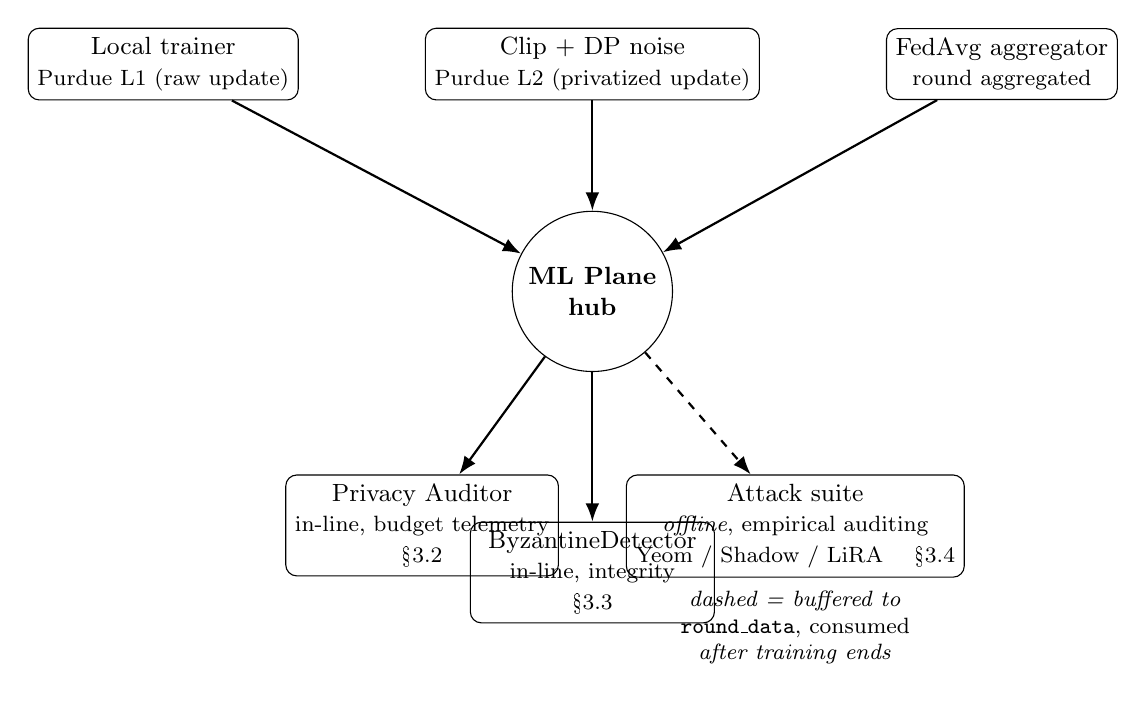
\begin{tikzpicture}[
  node distance=1.1cm and 1.6cm,
  box/.style={draw, rounded corners, minimum height=0.9cm, minimum width=2.6cm, align=center, font=\small},
  hub/.style={draw, circle, minimum size=1.3cm, align=center, font=\small\bfseries},
  consumer/.style={draw, rounded corners, minimum height=1.1cm, minimum width=3.1cm, align=center, font=\small},
  arr/.style={-Latex, thick}
]
  % Purdue-level producers
  \node[box] (local) {Local trainer\\\footnotesize Purdue L1 (raw update)};
  \node[box, right=of local] (privatize) {Clip + DP noise\\\footnotesize Purdue L2 (privatized update)};
  \node[box, right=of privatize] (aggregate) {FedAvg aggregator\\\footnotesize round aggregated};

  % Hub
  \node[hub, below=1.4cm of privatize] (hub) {ML Plane\\hub};

  % Three consumers
  \node[consumer, below left=1.6cm and -0.3cm of hub] (auditor) {Privacy Auditor\\\footnotesize in-line, budget telemetry\\\footnotesize \S3.2};
  \node[consumer, below=1.9cm of hub] (byz) {ByzantineDetector\\\footnotesize in-line, integrity\\\footnotesize \S3.3};
  \node[consumer, below right=1.6cm and -0.3cm of hub] (attacks) {Attack suite\\\footnotesize \emph{offline}, empirical auditing\\\footnotesize Yeom / Shadow / LiRA \quad \S3.4};

  \draw[arr] (local) -- (hub);
  \draw[arr] (privatize) -- (hub);
  \draw[arr] (aggregate) -- (hub);

  \draw[arr] (hub) -- (auditor);
  \draw[arr] (hub) -- (byz);
  \draw[arr, dashed] (hub) -- (attacks);

  % Nota: \\ non deve mai comparire dentro l'argomento di \emph{...} in un
  % nodo TikZ con align=center -- TikZ intercetta \\ per l'allineamento
  % tabellare del testo del nodo e un \\ annidato in un altro comando causa
  % "Undefined control sequence \pgfutil@next" (verificato isolando il bug
  % in una compilazione di prova, 2026-09-15). Per questo qui \emph si
  % applica riga per riga, con i \\ sempre al livello esterno.
  \node[font=\footnotesize, below=0.05cm of attacks, align=center] {\emph{dashed = buffered to}\\\texttt{round\_data}, consumed\\\emph{after training ends}};

\end{tikzpicture}
\caption{The ML Plane publishes three Purdue-labeled event types per
round to a central hub, which fans them out to three independent
consumers. The Privacy Auditor and ByzantineDetector process events
in-line, without altering the training loop; the attack suite buffers
the same events and runs offline, after training completes
(Section~\ref{sec:framework-attacks}).}
\label{fig:mlplane}
\end{figure}

\begin{figure}[t]
\centering
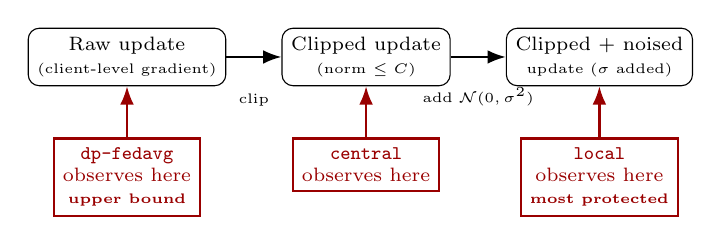
\begin{tikzpicture}[
  node distance=0.5cm,
  stage/.style={
    draw,
    rounded corners,
    minimum height=0.7cm,
    minimum width=1.9cm,
    align=center,
    font=\scriptsize
  },
  tap/.style={
    draw,
    -Latex,
    thick,
    red!60!black
  },
  arr/.style={-Latex, thick}
]

  \node[stage] (raw)
    {Raw update\\\tiny (client-level gradient)};

  \node[stage, right=0.70cm of raw] (clip)
  {Clipped update\\\tiny (norm $\le C$)};

\node[stage, right=0.70cm of clip] (noise)
  {Clipped + noised\\\tiny update ($\sigma$ added)};

  \draw[arr] (raw) --
  node[above=-0.75cm, font=\tiny]{clip} (clip);

 \draw[arr] (clip) --
  node[above=-0.75cm, font=\tiny]{add $\mathcal{N}(0,\sigma^2)$} (noise);

  \node[tap, below=0.65cm of raw,
        font=\scriptsize, align=center] (dpfedavg)
    {\texttt{dp-fedavg}\\observes here\\\tiny \textbf{upper bound}};

  \node[tap, below=0.65cm of clip,
        font=\scriptsize, align=center] (central)
    {\texttt{central}\\observes here};

  \node[tap, below=0.65cm of noise,
        font=\scriptsize, align=center] (local)
    {\texttt{local}\\observes here\\\tiny \textbf{most protected}};

  \draw[tap] (dpfedavg) -- (raw);
  \draw[tap] (central) -- (clip);
  \draw[tap] (local) -- (noise);

\end{tikzpicture}
\caption{The three DP placements evaluated in this paper are three
points of adversary privilege along one pipeline, not three privacy
mechanisms. \texttt{dp-fedavg} sees the raw update and is the upper
bound on extractable signal; \texttt{central} sees the clipped update
before noise; \texttt{local} sees only the final, noised update. If the
upper-bound placement shows no attack signal, a null result under the
protective placements cannot be attributed to noise suppressing an
otherwise-present signal (Section~\ref{sec:framework-dp}).}
\label{fig:dp-placements}
\end{figure}
% ChargeShield-FL --- DSN 2027 --- Figura: i tre punti di osservazione
% dell'avversario (2026-09-16, Sprint 10zz+117).
%
% NOTA TIKZ: ogni \\ deve restare al livello ESTERNO del testo del nodo. Un
% \\ annidato dentro l'argomento di un altro comando (es. \emph{a\\b}) rompe
% il layout di align con "Undefined control sequence \pgfutil@next" --- bug
% reale trovato e corretto nel Sprint 10zz+109 su ml_plane_architecture.tex.
\begin{figure}[t]
\centering
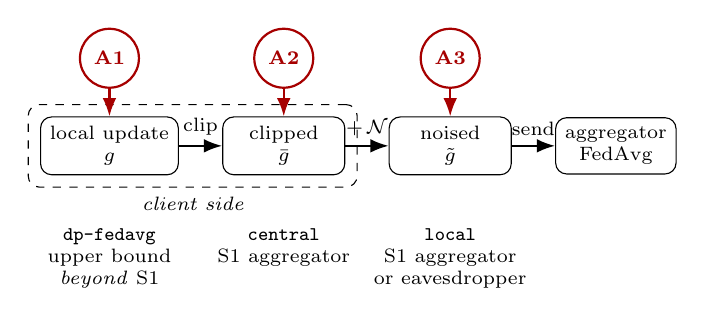
\begin{tikzpicture}[
 font=\footnotesize,
  stage/.style={draw, rounded corners, minimum height=0.65cm,
                minimum width=1.55cm, align=center, font=\scriptsize},
  zone/.style={draw, dashed, rounded corners, inner sep=0.15cm},
  adv/.style={draw, circle, minimum size=0.48cm, thick,
              red!65!black, font=\scriptsize\bfseries},
  arr/.style={-Latex, thick}
]

  \node[stage] (raw)   {local update\\$g$};
  \node[stage, right=0.55cm of raw]  (clip)  {clipped\\$\bar{g}$};
  \node[stage, right=0.55cm of clip] (noise) {noised\\$\tilde{g}$};
  \node[stage, right=0.55cm of noise, minimum width=1.4cm] (agg) {aggregator\\FedAvg};

  \draw[arr] (raw)   -- node[above, font=\scriptsize]{clip} (clip);
  \draw[arr] (clip)  -- node[above, font=\scriptsize]{$+\,\mathcal{N}$} (noise);
  \draw[arr] (noise) -- node[above, font=\scriptsize]{send} (agg);

  % zona che non lascia mai il client
  \begin{scope}[on background layer]
    \node[zone, fit=(raw)(clip), label={[font=\scriptsize\itshape]below:client side}] {};
  \end{scope}

  \node[adv, above=0.35cm of raw]   (a1) {A1};
  \node[adv, above=0.35cm of clip]  (a2) {A2};
  \node[adv, above=0.35cm of noise] (a3) {A3};
  \draw[arr, red!65!black] (a1) -- (raw);
  \draw[arr, red!65!black] (a2) -- (clip);
  \draw[arr, red!65!black] (a3) -- (noise);

  \node[font=\scriptsize, align=center, below=0.55cm of raw]   {\texttt{dp-fedavg}\\upper bound\\\emph{beyond} S1};
  \node[font=\scriptsize, align=center, below=0.55cm of clip]  {\texttt{central}\\S1 aggregator};
  \node[font=\scriptsize, align=center, below=0.55cm of noise] {\texttt{local}\\S1 aggregator\\or eavesdropper};

\end{tikzpicture}
\caption{The three observation points are three adversary privileges on one
privatisation pipeline, not three privacy mechanisms. \textbf{A3} sees only
the clipped-and-noised update: an honest-but-curious aggregator, or a network
observer, under a local-DP deployment. \textbf{A2} sees the update after
clipping but before noise, which is what an aggregator legitimately receives
when the noise is added centrally --- still Scenario~1. \textbf{A1} sees the
raw update, which under our deployments never leaves the client
unprivatised; it therefore models an adversary \emph{strictly stronger} than
Scenario~1, and we evaluate it precisely because a null there bounds the
other two (\S\ref{sec:threat-observation}).}
\label{fig:adversary-points}
\end{figure}


\bibliographystyle{IEEEtran}
\bibliography{references}

\end{document}
